\documentclass[aspectratio=169]{beamer}
\geometry{paperwidth=160mm,paperheight=100mm}
\usepackage{beamerthemesidebar}
\usepackage{hyperref}
\usepackage{color}
\usepackage{multimedia}
\usepackage{colortbl}
\usepackage{amsmath}
\usepackage{empheq}
\usepackage{cancel}
\usepackage{amssymb}
\usepackage{amsfonts}
\usepackage{lipsum}
\usepackage{tcolorbox}
\usepackage{tabularx}
\usepackage{caption}
\usepackage{bm}

\setbeamersize{sidebar width right=0pt}
\setbeamertemplate{footline}[frame number]
%
\definecolor{orange}{RGB}{250,167,12}
\definecolor{yellow}{RGB}{246,250,12}
\definecolor{green}{RGB}{128,238,1}
\definecolor{black}{RGB}{0,0,0}
\definecolor{blue}{RGB}{0,0,255}
\definecolor{red}{RGB}{255,0,0}
\definecolor{sepia}{RGB}{94,38,18}
\newcommand{\ve}[1]{{\rm\bf {#1}}}
\newcommand{\q}[1]{\textcolor{blue}{#1}}
\newcommand{\blue}[1]{\textcolor{blue}{#1}}
\newcommand{\sepia}[1]{\textcolor{sepia}{#1}}
\newcommand{\red}[1]{\textcolor{red}{#1}}
\newcommand{\green}[1]{\textcolor{green}{#1}}
\newcommand{\yellow}[1]{\textcolor{yellow}{#1}}
\newcommand{\orange}[1]{\textcolor{orange}{#1}}
\definecolor{burlywood}{RGB}{255,211,155}
\definecolor{chocolate}{RGB}{255,127,36}
\definecolor{tan}{RGB}{210,180,140}
%
\def\onethird{{\textstyle{1\over3}}}
\def\twothirds{{\textstyle{2\over3}}}
\def\fourthirds{{\textstyle{4\over3}}}
\def\onehalf{{\textstyle{1\over2}}}
\def\threehalfs{{\textstyle{3\over2}}}
%
\newcommand{\pd}{\partial}
\newcommand{\aMLT}{\alpha_{\rm MLT}}
\newcommand{\Fconv}{F_{\rm conv}}
\newcommand{\Frad}{F_{\rm rad}}
\newcommand{\Ftot}{F_{\rm tot}}
\newcommand{\Hp}{H_p}
\newcommand{\prad}{p_{\rm rad}}
\newcommand{\pgas}{p_{\rm gas}}
\newcommand{\TTc}{T_{\rm c}}
\newcommand{\rhoc}{\rho_{\rm c}}
\newcommand{\Teff}{T_{\rm eff}}
\newcommand{\Fstar}{F_\star}
\newcommand{\pstar}{p_\star}
\newcommand{\Pstar}{P_\star}
\newcommand{\Rstar}{R_\star}
\newcommand{\rhostar}{\rho_\star}
\newcommand{\Tstar}{T_\star}
%
\title{Theoretical Astrophysics I: Physics of Sun and Stars\\
Lecture 10: The Sun}
\author{\texorpdfstring{\sepia{Petri K\"{a}pyl\"{a} Ivan Mili\'{c}}\newline\blue{\url{pkapyla, milic@leibniz-kis.de}}}{}}
\institute{Institut f\"ur Sonnenphysik - KIS, Freiburg}
\date{\today}
%
\begin{document}
\frame{\titlepage}


\section{Recap and intro}
%
\frame{
\frametitle{Recap}
\begin{itemize}
\item We talked about the interior of the stars, their spectra and their evolution. 
\item We now have a rough understanding about what the stars do (they shine).
\item Now we turning to an obvious example of a star: The Sun. 
\item We will discuss a group of somewhat disjointed topics about the Sun - the goal is to present you the solar science but also to outline what makes the Sun unique. 
\item \textbf{Probably nothing - Sun is a fairly ordinary star. But for science - it is absolutely priceless.}
\end{itemize}
}
%
%
\frame{
\frametitle{Why is the Sun important?}
\begin{minipage}{0.54\linewidth}
\begin{itemize}
\item Obviously, sunlight is important for sustaining life. 
\item But also, increased emission of high energy photons due violent explosive processes can be threatening for life on Earth.
\item Magnetic fields of the Sun interact with our magnetic fields (geomagnetic storms). 
\item There are also occasional bursts of charged particles emerging from the Sun and reaching the Earth. 
\item All this is called: \textbf{space weather}.
\end{itemize}
\end{minipage}
\begin{minipage}{0.45\linewidth}
\begin{figure}
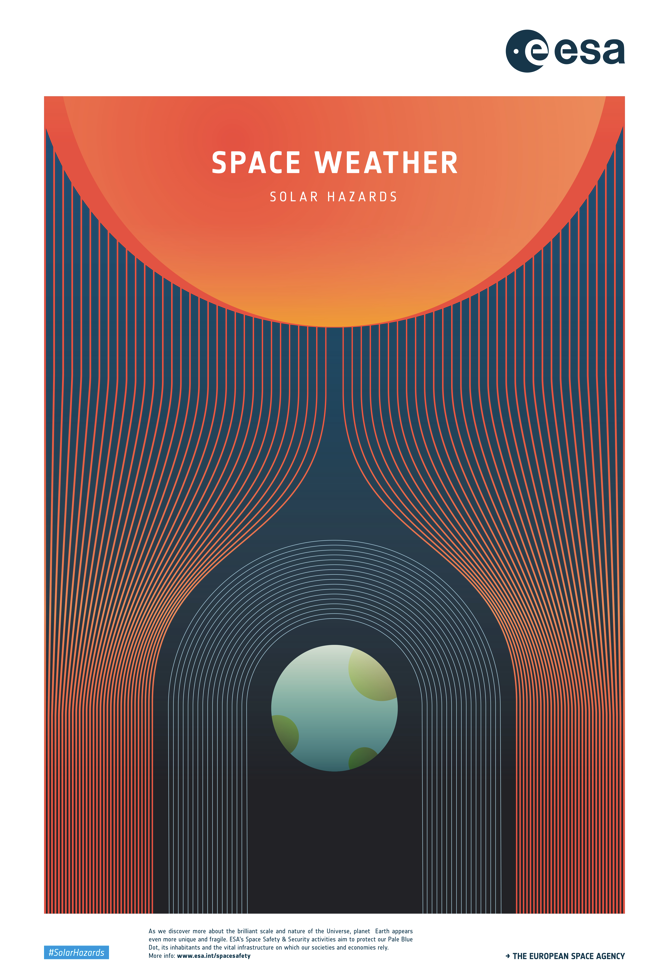
\includegraphics[width=6cm]{figures/sw_poster.png}
\caption*{Credits: ESA}
\end{figure}
\end{minipage}
}
%
%
\frame{
\frametitle{Why is the Sun important?}
\begin{minipage}{0.54\linewidth}
\begin{itemize}
\item On the other hand - Sun is (almost) the only star that we can resolve. 
\item Perfect testbed for testing our theories about stellar structure, evolution, stellar atmosphere theory. 
\item Also for plasma physics, turbulence, reconnection, magnetohydrodynamics.
\item Understanding the interaction between Sun and the Earth is the key to understanding exoplanets. 
\item Overall - understanding Sun better allows us to apply this knowledge (and the techniques to other fields of astrophysics).
\end{itemize}
\end{minipage}
\begin{minipage}{0.45\linewidth}
\begin{figure}
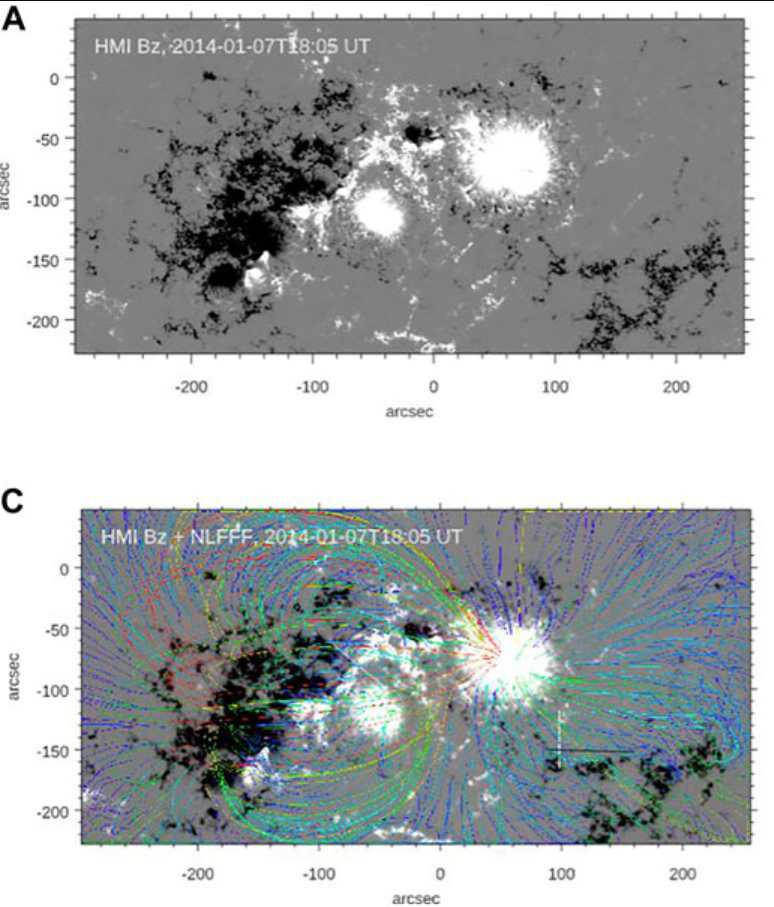
\includegraphics[width=6cm]{figures/extrapolations.png}
\caption*{Credits: Yurchyshyn et al., 2022}
\end{figure}
\end{minipage}
}
%
%
%
\frame{
\frametitle{Relationship between solar physics and astrophysics}
These are some of the overlaps or common interests: 
\begin{itemize}
\item Spectroscopy/spectropolarimetry: essential to probe physical conditions in the solar/stellar/planetary atmospheres.
\item Helio(astro)seismology: probing the interior regions of Sun and stars. 
\item Stellar structure and stellar atmospheres: Sun was the first test for these theories. 
\item Solar and stellar activity: flares, chromospheric events, prominences, etc. also happen on other stars.  
\item Physics of hot and ionized plasmas: conditions in solar transition region / corona are similar to the conditions in AGN enviroments, HII regions, and other nebulae.
\item \textbf{And probably more that I am simply not aware of :-)}
\end{itemize}
}
%
\section{Importance of high resolution}
%
\frame{
\frametitle{How well can we really see the Sun?}
\begin{minipage}{0.52\linewidth}
\begin{itemize}
\item Right: solar granulation captured by DKIST solar telescope (4m, credits: NSO/NSF/AURA)
\item Many questions for you:
\item \q{How big would you say is one pixel at the image?}
\item \q{How many photons does one pixel emit per second?}
\item \q{How many of these photons reach the DKIST telescope?}
\end{itemize}
\end{minipage}
\begin{minipage}{0.47\linewidth}
\begin{figure}
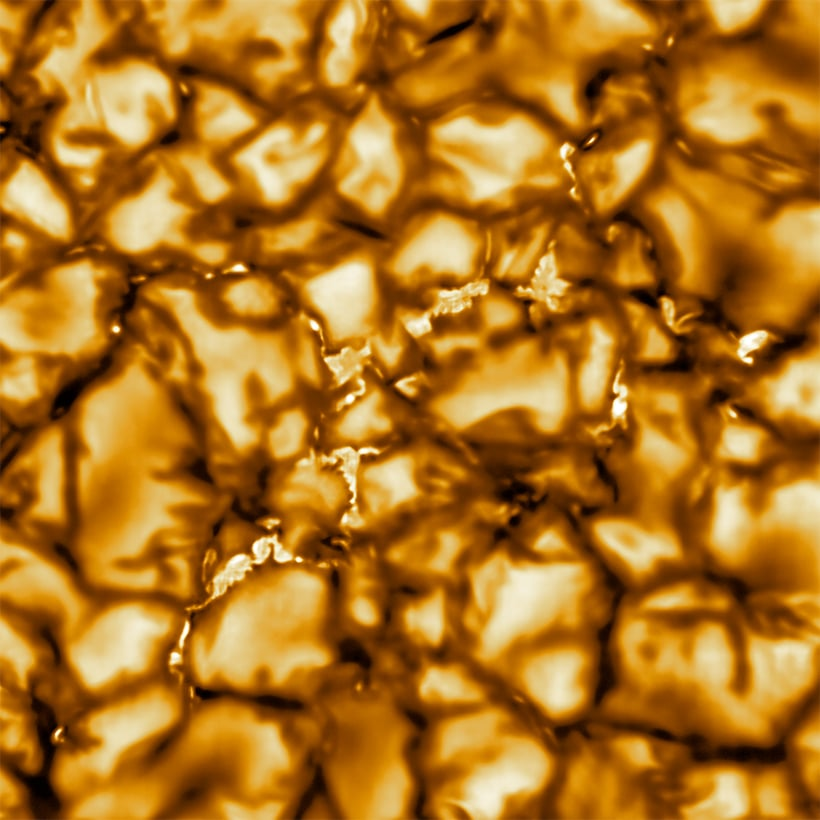
\includegraphics[width=6cm]{figures/dkist_big.jpg}
\caption*{Credits: NSO/DKIST/NSF/AURA}
\end{figure}
\end{minipage}
}
%
%
\frame{
\frametitle{How well can we really see the Sun?}
\begin{minipage}{0.52\linewidth}
\begin{itemize}
\item Right: solar granulation captured by DKIST solar telescope (4m, credits: NSO/NSF/AURA)
\item Many questions for you:
\item Diffraction limit of this telescope in visible is around 30\,km, so these pixels should correspond to around 15\,km.
\item Apply blackbody law and multiply with the surface of one pixel, number should be huge!
\item Apply the blackbody law and find the intensity, then multiply with the solid angle corresponding to surface of DKIST mirror seen from the Sun, number should be much smaller.
\end{itemize}
\end{minipage}
\begin{minipage}{0.47\linewidth}
\begin{figure}
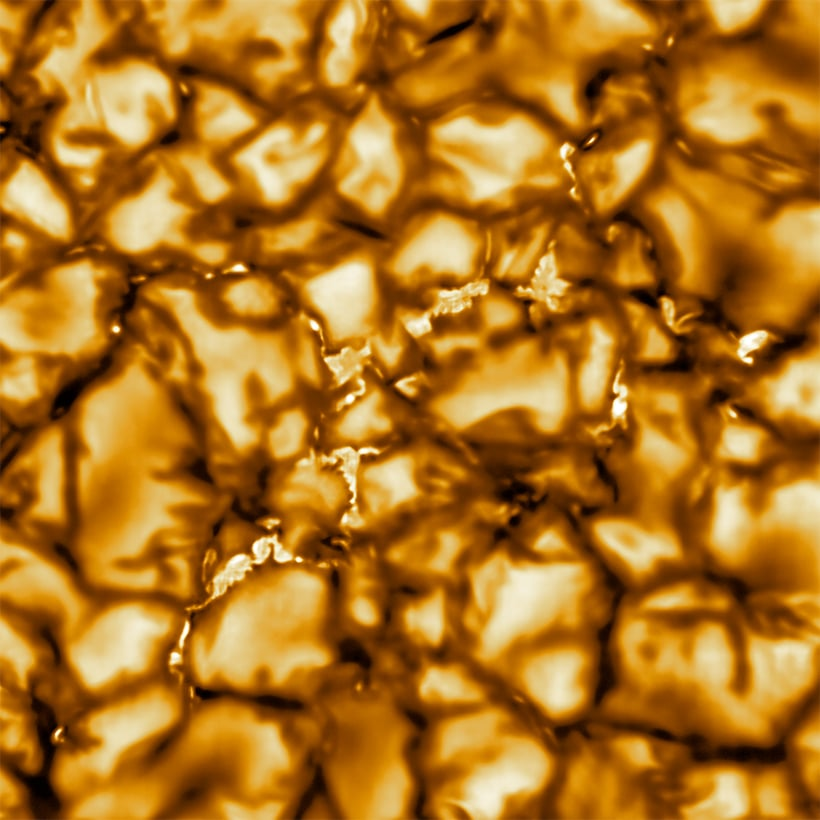
\includegraphics[width=6cm]{figures/dkist_big.jpg}
\caption*{Credits: NSO/DKIST/NSF/AURA}
\end{figure}
\end{minipage}
}
%
%
\frame{
\frametitle{Solar spectrum}
\begin{figure}
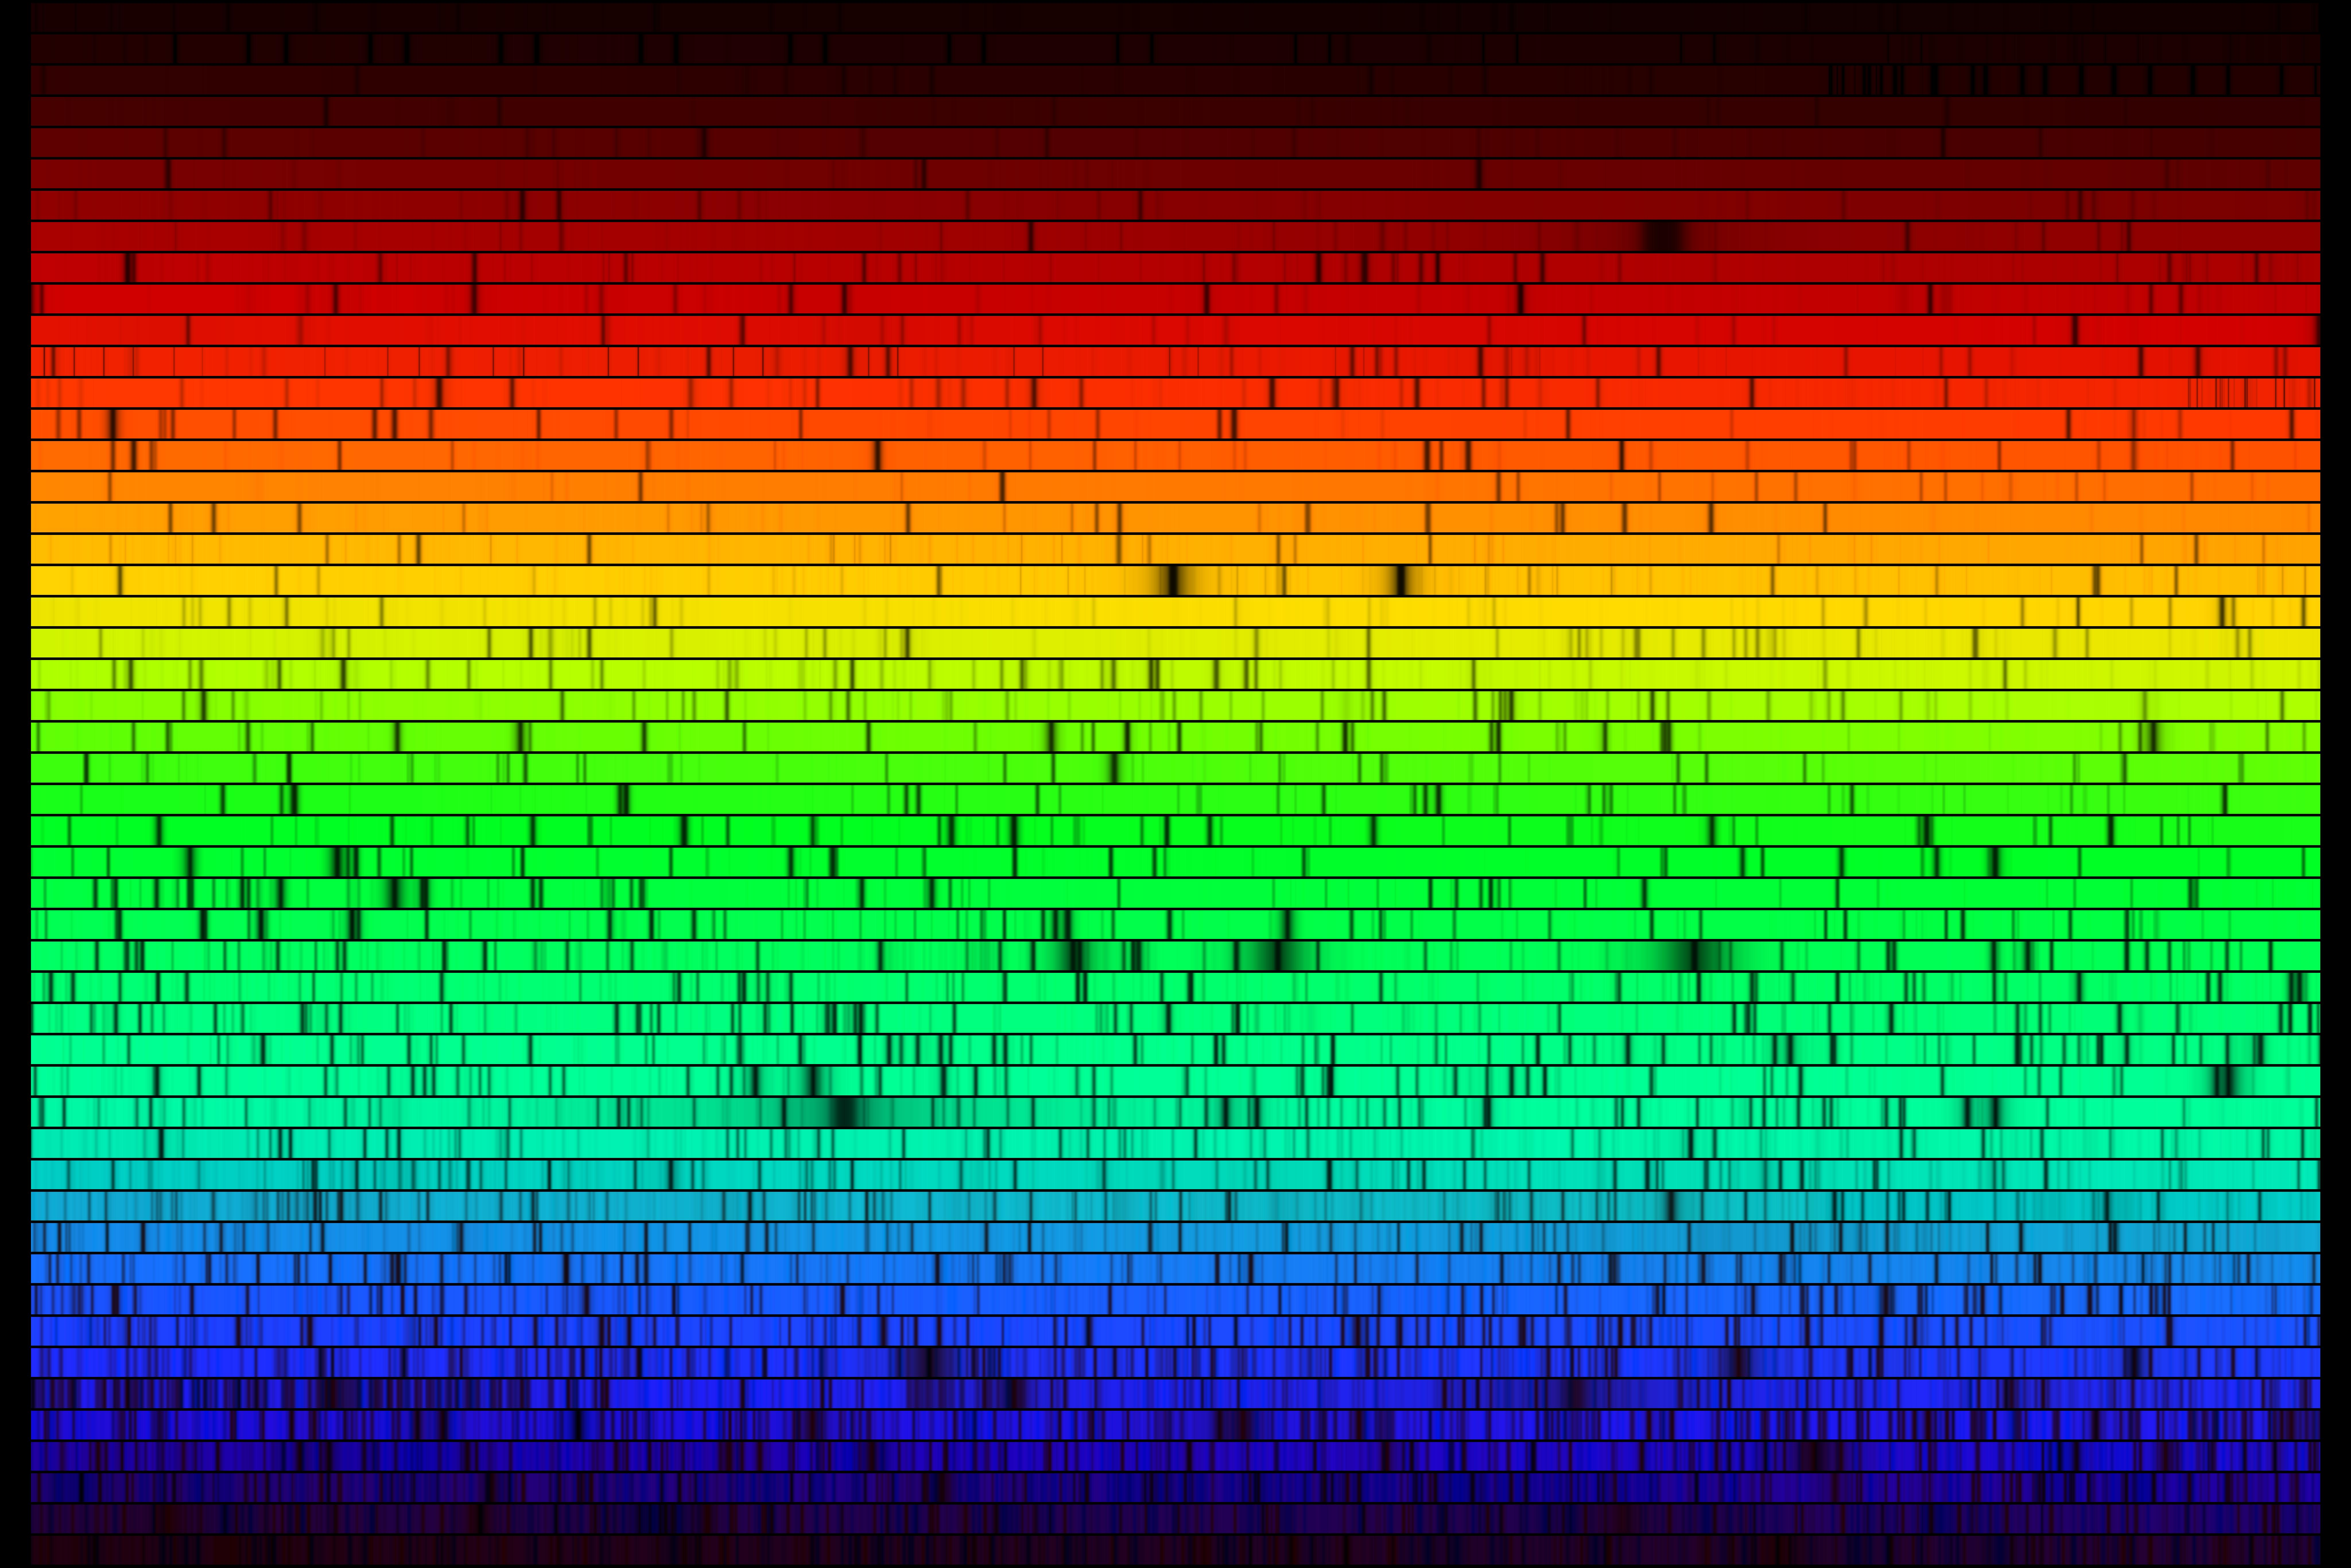
\includegraphics[width=11cm]{figures/solarspectrum.jpg}
\caption*{Solar Spectrum. Credits: N.A.Sharp, NOAO/NSO/Kitt Peak FTS/AURA/NSF}
\end{figure}
}
%
%
\frame{
\frametitle{Solar spectral lines example}
\begin{figure}
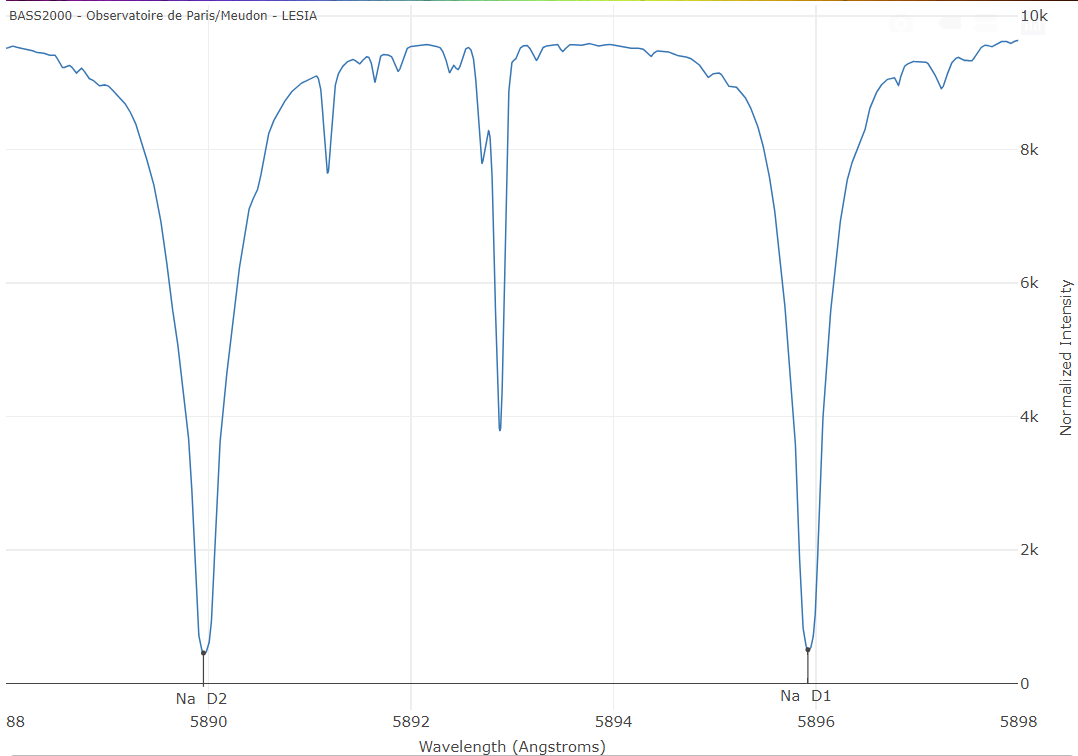
\includegraphics[width=11cm]{figures/na_D.png}
\caption*{Sodium D lines in the solar spectrum. Credits: BASS2000}
\end{figure}
}
%
\frame{
\frametitle{Spectral lines: bound-bound processes}
\begin{minipage}{0.52\linewidth}
\begin{itemize}
\item Finally, we can talk about the absorption and emission between two bound states. 
\item This gives rise to the spectral line processes. 
\item There, the opacity varies dramatically with wavelenght. We often write:
\begin{equation}
\kappa_\nu = \kappa_0 \phi_\nu
\end{equation}
\item $\phi_\nu$ is the \textbf{line absorption profile}. It varies very quickly with the wavelength.
\end{itemize}
\end{minipage}
\begin{minipage}{0.47\linewidth}
\begin{figure}
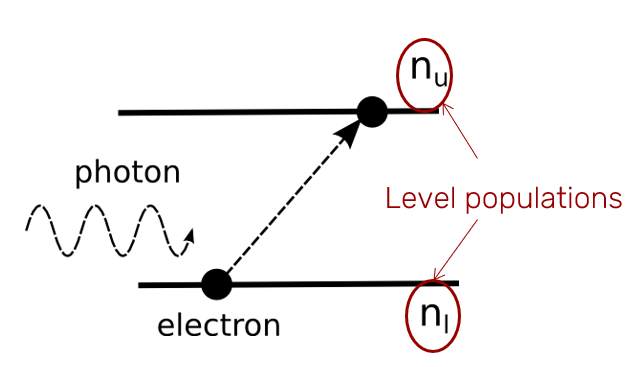
\includegraphics[width=6cm]{figures/spectralline.png}
\caption{The photon gets absorbed via bound-bound process. Excited atom then can deposit the energy back into the gas, or emit a new photon, similar to the old one.}
\end{figure}
\end{minipage}
}
%
%
\frame{
\frametitle{Spectral lines: line absorption profile}
\begin{minipage}{0.52\linewidth}
\begin{itemize}
\item In theory, spectral lines should be $\delta$-functions. In reality, delta function does not exist of course: 
\item First, there is an uncertainty in the energy, leading to a finite width of the energy levels. 
\item Then, there is perturbation of the energy levels by the environment. 
\item Then, the particles are moving and thus shifting their absorption profile toward blue and toward red, according to Maxwell velocity distribution, projected onto the line-of-sight:
\begin{equation}
p(v) = \frac{1}{\sqrt{\pi} v_D} e^{-v^2/ v_D^2}
\end{equation}
\end{itemize}
\end{minipage}
\begin{minipage}{0.47\linewidth}
\begin{figure}
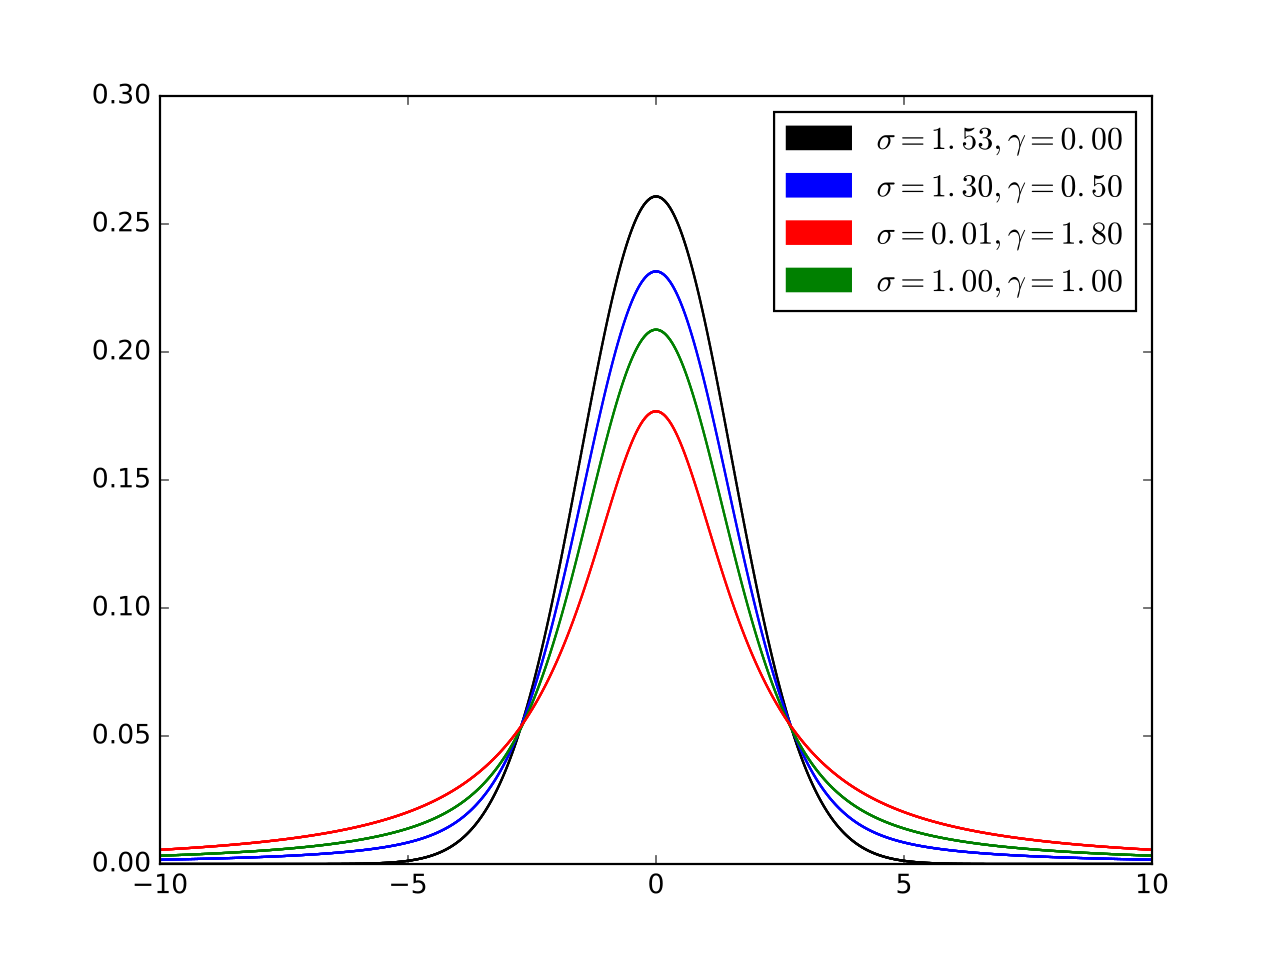
\includegraphics[width=6cm]{figures/voigt.png}
\caption*{Credits: Wikipedia}
\end{figure}
\end{minipage}
}
%
%
\frame{
\frametitle{Spectral lines: cross-section}
\begin{minipage}{0.52\linewidth}
\begin{itemize}
\item Similarly to the continuum processes, we can always write the opacity as something like: 
\begin{equation}
\kappa_0 = \frac{1}{\rho} n_{\rm lower} \sigma_0
\end{equation}
\item Where this $\sigma_0$ depends on the nature of the transition.
\item It can vary by orders of magnitude (strong spectral lines vs ``forbidden'' spectral lines).
\item \q{What else determines the strength of a spectral line?}
\end{itemize}
\end{minipage}
\begin{minipage}{0.47\linewidth}
\begin{figure}
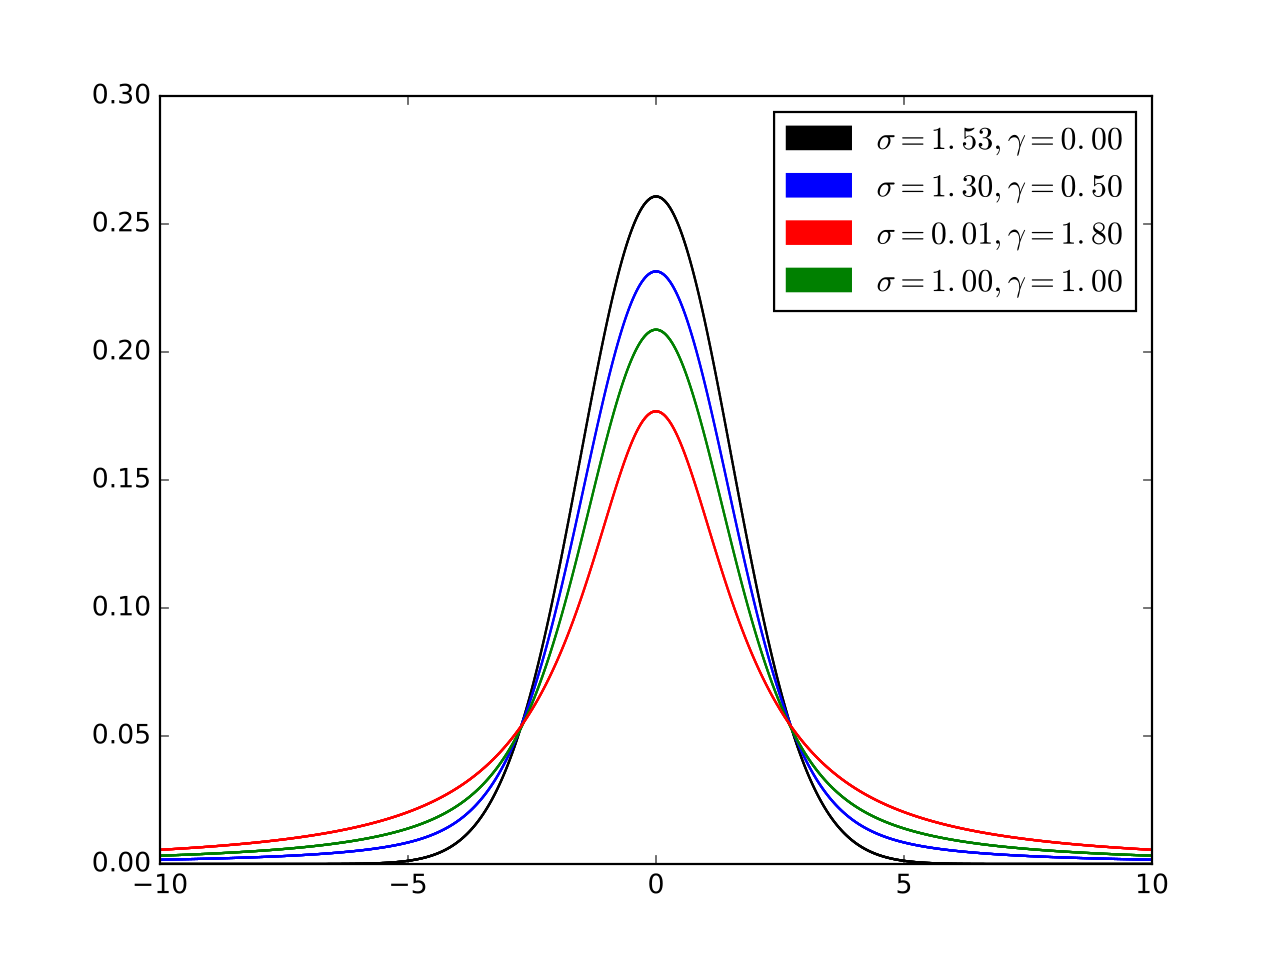
\includegraphics[width=6cm]{figures/voigt.png}
\caption*{Credits: Wikipedia}
\end{figure}
\end{minipage}
}
%
%
\frame{
\frametitle{Spectral lines: cross-section}
\begin{minipage}{0.52\linewidth}
\begin{itemize}
\item \q{What else determines the strength of a spectral line?}
\begin{equation}
\kappa_0 = \frac{1}{\rho} n_{\rm lower} \sigma_0
\end{equation}
\item The number density of the lower level of the transition! Recall the Boltzmann equation:
\begin{equation}
n_{i,j} = n_{j} \frac{g_i e^{-E_i/kT}}{Q_j}
\end{equation}
\item Here $n_j$ is the total population of that ion, and $Q_j$ is the partition function.
\item So, to have a strong line, we need an abundant element, with appropriate ionization state at a given temperature. 
\end{itemize}
\end{minipage}
\begin{minipage}{0.47\linewidth}
\begin{figure}
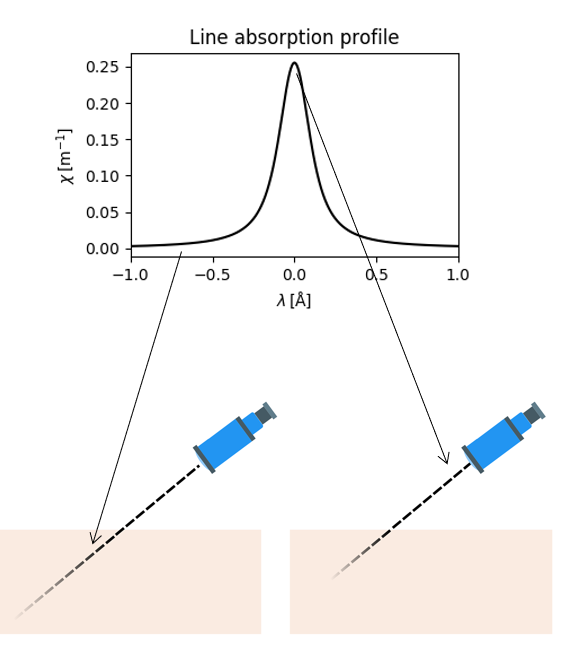
\includegraphics[width=6cm]{figures/line_depth.png}
\end{figure}
\end{minipage}
}
%
%
\frame{
\frametitle{Spectral lines: formation heights}
\begin{minipage}{0.52\linewidth}
\begin{itemize}
\item Stronger line - larger opacity - we see higher layers. We can define something called ``height of formation.''
\item This height gives us a rough idea what layers we see when we observe a specific wavelength in spectral line. 
\item Remember that different wavelengths in the same spectral line still probe different heights. 
\item So, even by probing one line only we can do the ``tomography'' of the solar atmosphere. 
 \end{itemize}
\end{minipage}
\begin{minipage}{0.47\linewidth}
\begin{figure}
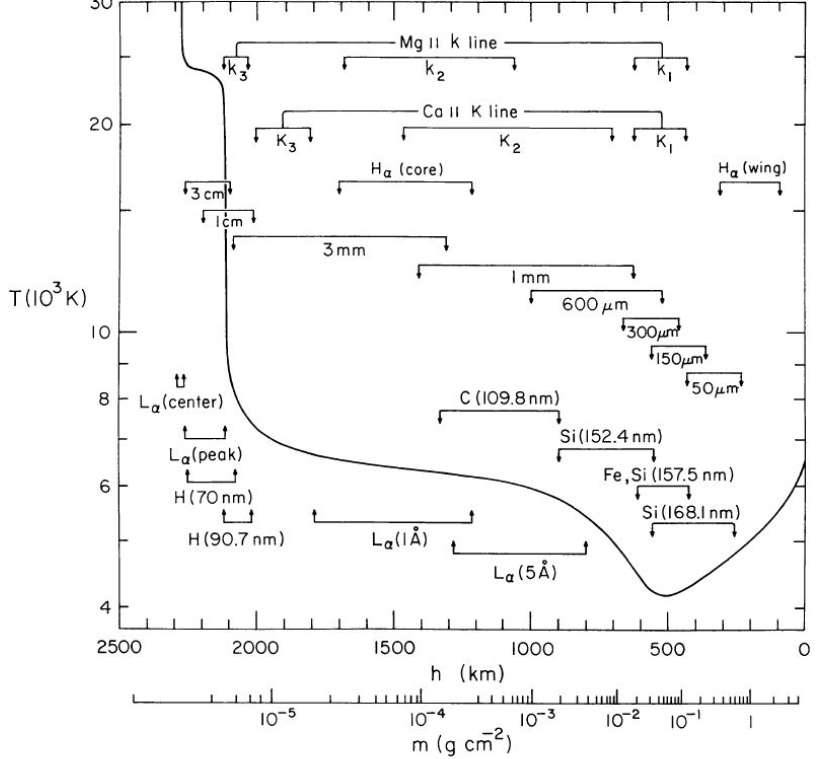
\includegraphics[width=6cm]{figures/vernazza.png}
\caption*{Credits: Vernazza et al. 1981}
\end{figure}
\end{minipage}
}
%
%
\frame{
\frametitle{Spectral lines: 3D information}
\begin{figure}
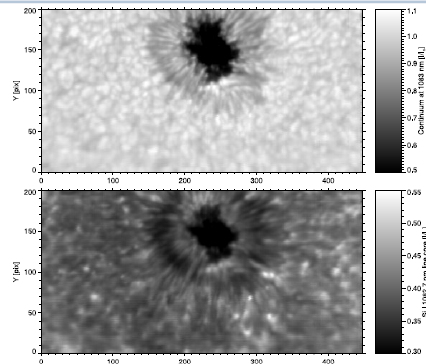
\includegraphics[width=6.5cm]{figures/gris1.png}
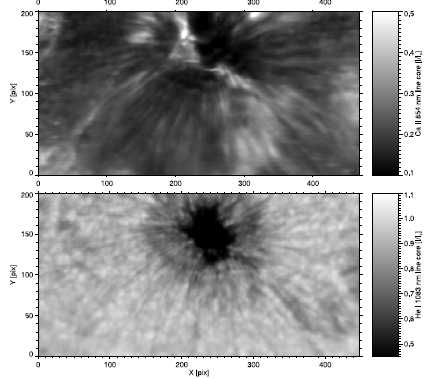
\includegraphics[width=6.5cm]{figures/gris2.png}
\caption*{Credits: GRIS team}
\end{figure}
}
%
%
\frame{
\frametitle{Spectral lines: Zeeman effect}
\begin{minipage}{0.52\linewidth}
\begin{itemize}
\item Around 1920, George Ellery Hale observed the spectrum of a nickel line in the Sun. 
\item When his spectrograph slit (\q{what is this?}) crossed the Sunspot - spectral line split. 
\item Not long ago, Pieter Zeeman got a Nobel prize for discovering exactly that. 
\item This was the first ``direct'' (not literally direct...) proof that Sunspots harbor magnetic fields! 
\item From the amount of splitting, one can infer the magnetic field. 
 \end{itemize}
\end{minipage}
\begin{minipage}{0.47\linewidth}
\begin{figure}
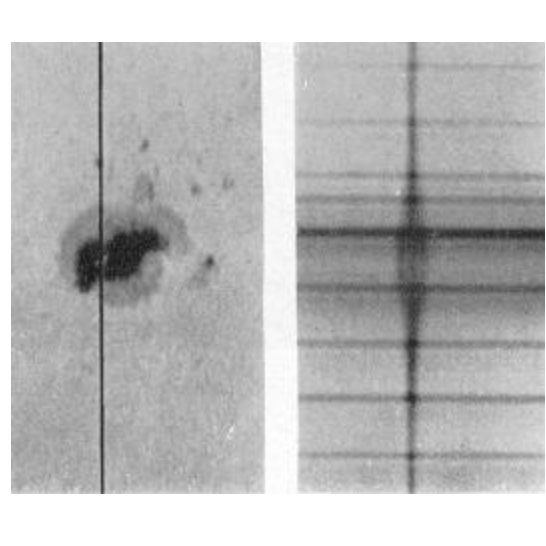
\includegraphics[width=6.5cm]{figures/hale.png}
\caption*{Credits: Mount Wilson Observatory}
\end{figure}
\end{minipage}
}
%
%
\frame{
\frametitle{Spectral lines: Polarization}
\begin{minipage}{0.52\linewidth}
\begin{itemize}
\item Today we use spectral line observations to infer the full magnetic field vector. 
\item The magnetic field polarizes the light at the wavelengths corresponding to a spectral line. 
\item Different sub-transitions have different polarizations. 
\item They get split in the wavelength so the polarization does not cancel. 
\item More about this in the next semester!
 \end{itemize}
\end{minipage}
\begin{minipage}{0.47\linewidth}
\begin{figure}
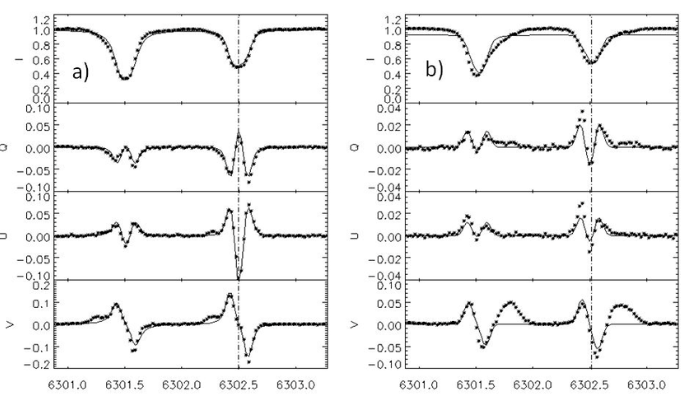
\includegraphics[width=7.5cm]{figures/borrero.png}
\caption*{Credits: Borrero \& Ichimoto (2011)}
\end{figure}
\end{minipage}
}
%
\section{Solar magnetic cycle}
%
\frame{
\frametitle{Counting sunspots}
\begin{minipage}{0.52\linewidth}
\begin{itemize}
\item Even before people have proven that the sunspots are magnetic, they have been counting them. 
\item First one was Horrebow, from roughly 1750. 
\item Schwabe discovered a regularity and Wolf introduced so-called Wolf's number (mid 1800s). 
\item When you look at it now - it's obvious, the Sunspots vary with a period of \textbf{11 years}.
\item This is the famous \textbf{solar activity cycle}.
\item Sunspots are magnetic formations, so this means the solar magnetic configuration changes with cycle.
 \end{itemize}
\end{minipage}
\begin{minipage}{0.47\linewidth}
\begin{figure}
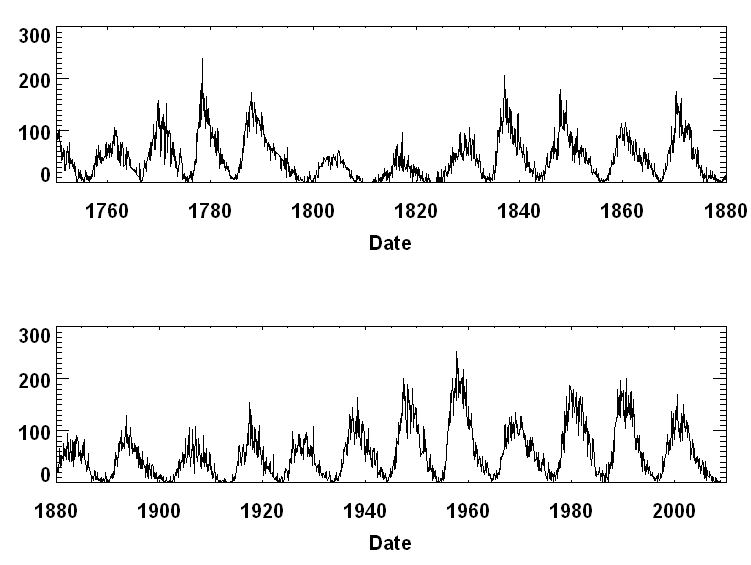
\includegraphics[width=6.5cm]{figures/issn.png}
\caption*{International sunspot number, credits: spaceweather.com}
\end{figure}
\end{minipage}
}
%
\frame{
\frametitle{Butterfly diagram}
\begin{minipage}{0.52\linewidth}
\begin{itemize}
\item The next step would be to follow the location of the sunspots on the disk. 
\item \q{Can you tell me how the spots move over the cycle?}
\end{itemize}
\end{minipage}
\begin{minipage}{0.47\linewidth}
\begin{figure}
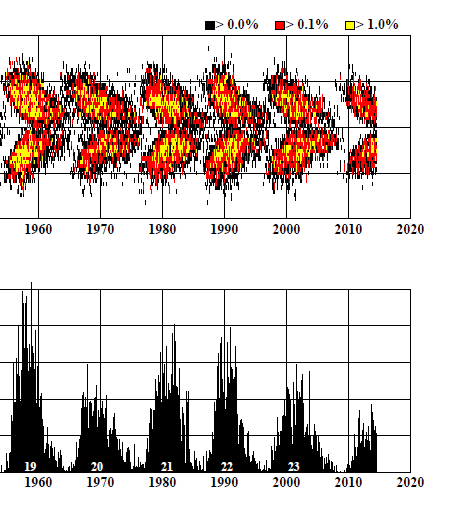
\includegraphics[width=6.5cm]{figures/butterfly.png}
\caption*{Credits: NASA/MSFC Hathaway}
\end{figure}
\end{minipage}
}
%
%
\frame{
\frametitle{Butterfly diagram}
\begin{minipage}{0.52\linewidth}
\begin{itemize}
\item The next step would be to follow the location of the sunspots on the disk. 
\item The spots appear on higher latitudes. 
\item Over the cycle they move more toward the equator. 
\item Eventually there are no more sunspots. 
\item The butterfly diagram is a reflection of what happens on the inside.
\end{itemize}
\end{minipage}
\begin{minipage}{0.47\linewidth}
\begin{figure}
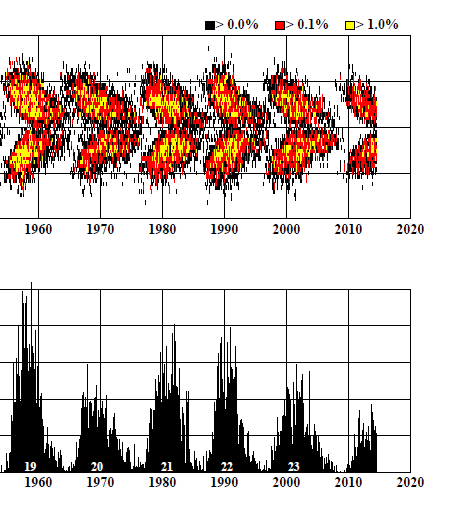
\includegraphics[width=6cm]{figures/butterfly.png}
\caption*{Credits: Hathaway, 2015}
\end{figure}
\end{minipage}
}
%
%
\frame{
\frametitle{Solar dynamo - schematic picture}
The interaction between magnetic fields and plasma flows periodically changes the topology of the magnetic fields.
\begin{figure}
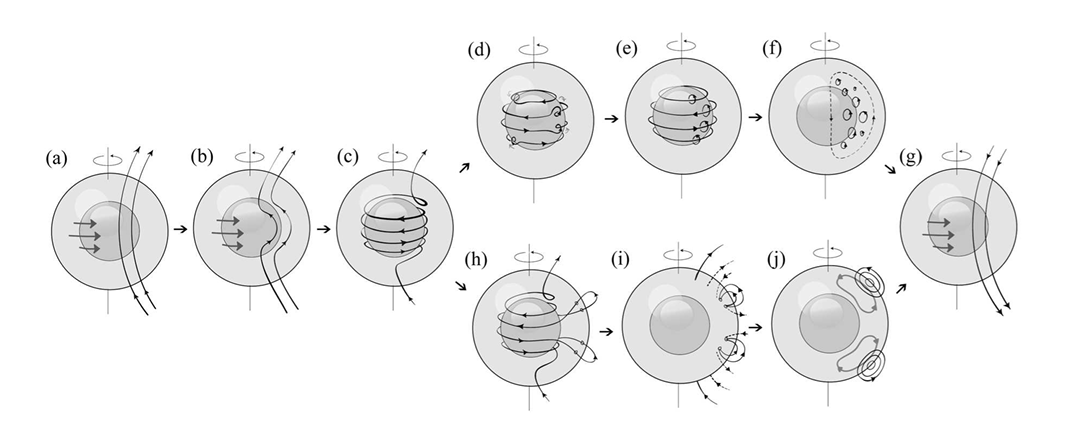
\includegraphics[width=14cm]{figures/sanchez_2013.png}
\caption*{Credits: Sanchez, 2013}
\end{figure}
}
%
%
\frame{
\frametitle{Solar cycle - the magnetic field}
The interaction between magnetic fields and plasma flows periodically changes the topology of the magnetic fields. We can also see that in the solar corona. 
\begin{figure}
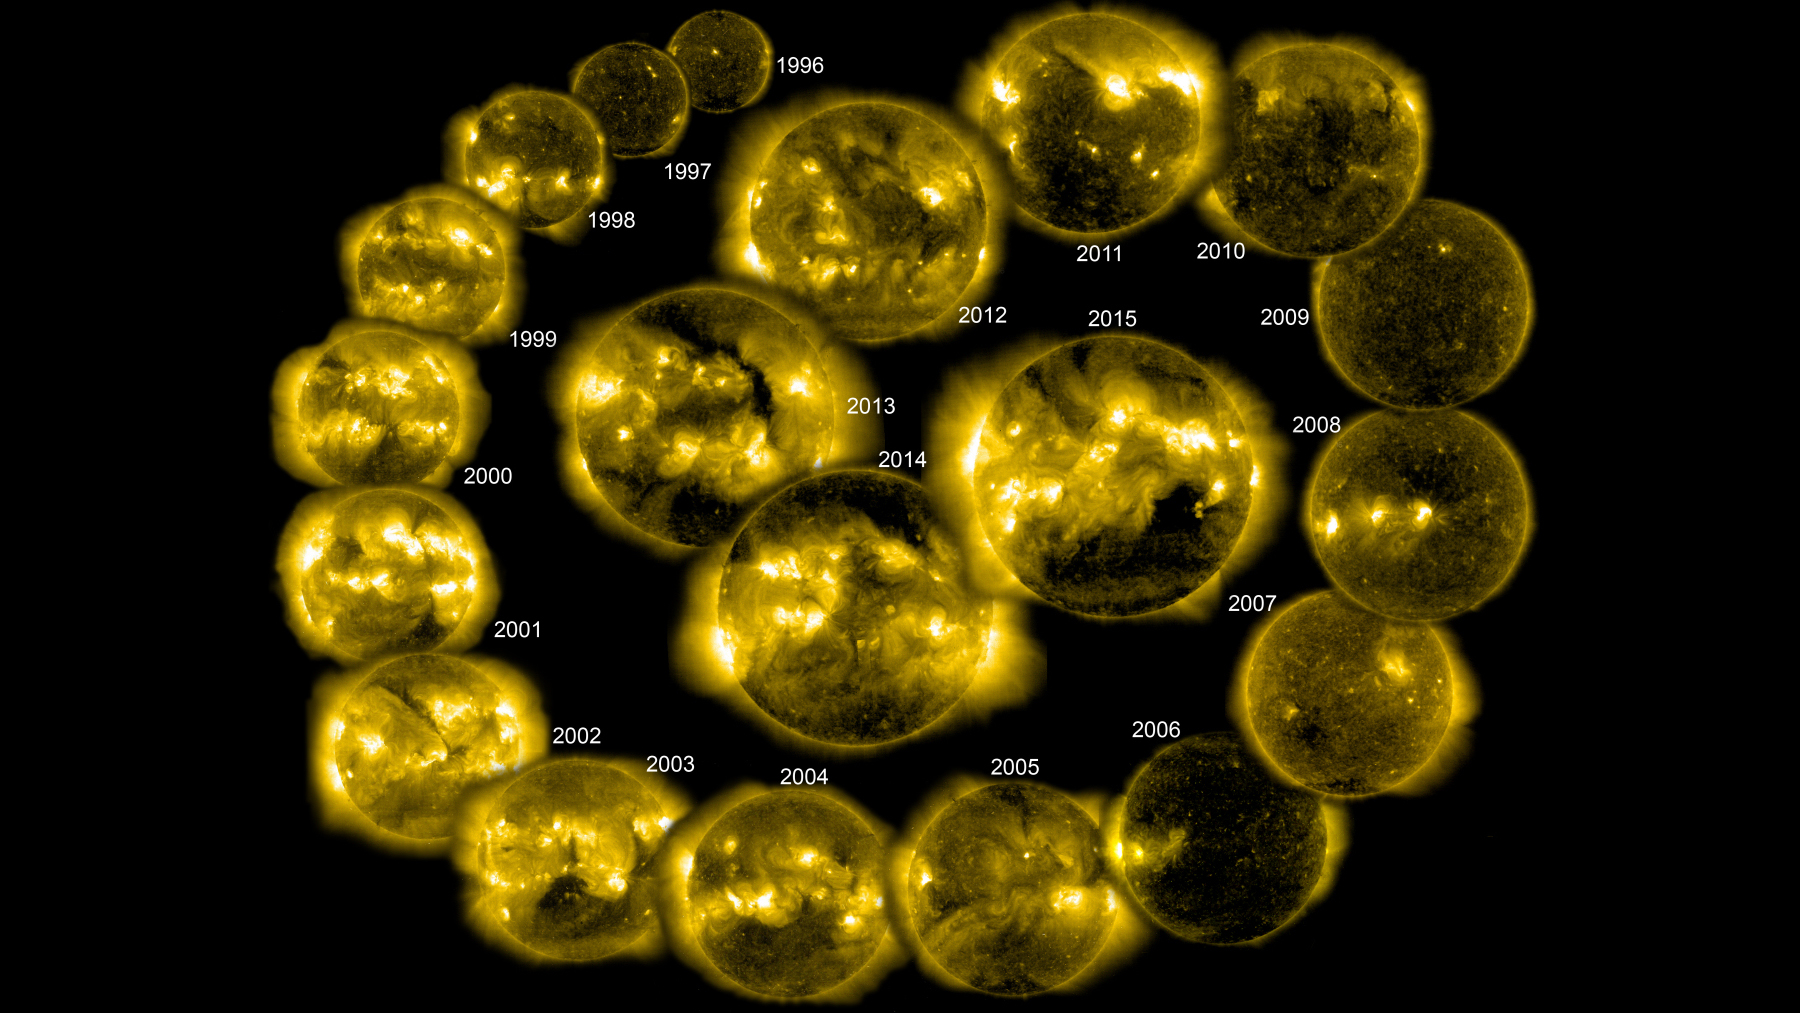
\includegraphics[width=12cm]{figures/aia_cycle.jpg}
\caption*{Credits: SDO/AIA, NASA}
\end{figure}
}
%
\section{Solar corona, filaments, and prominences}
%
\frame{
\frametitle{Solar Corona}
\begin{minipage}{0.52\linewidth}
\begin{itemize}
\item A hot ($>10^6$\,K) very thin (low density) layer of the solar atmosphere. 
\item Most of the elements are ionized to a very high degree.
\item Because the density is so low - the plasma follows the magnetic field. 
\item It is much more inhomogeneous and dynamic than the photosphere.
\item The coronal magnetic field can be understood through an extrapolation of the photospheric field.
\end{itemize}
\end{minipage}
\begin{minipage}{0.47\linewidth}
\begin{figure}
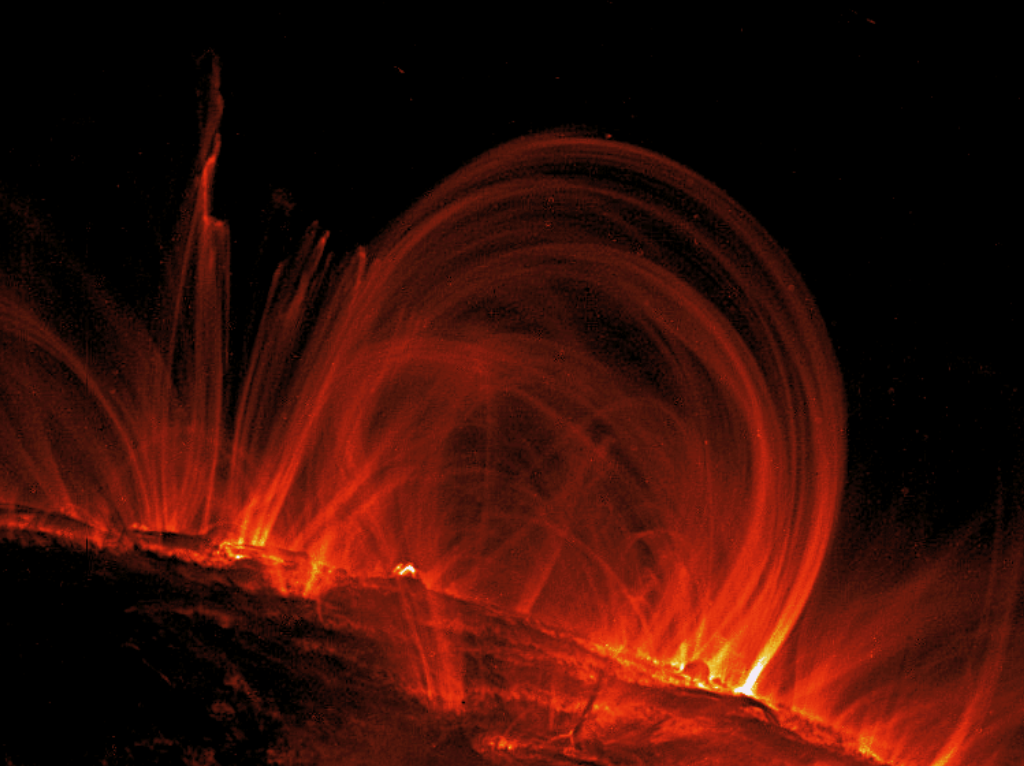
\includegraphics[width=6cm]{figures/trace_loops.png}
\caption*{Credits: TRACE/NASA}
\end{figure}
\end{minipage}
}
%
%
\frame{
\frametitle{Solar Corona - 1D picture}
\begin{minipage}{0.52\linewidth}
\begin{itemize}
\item A hot ($>10^6$\,K) very thin (low density) layer of the solar atmosphere. 
\item Most of the elements are ionized to a very high degree.
\item In a canonical 1D picture - there is a very narrow region where the density and temperature change dramatically - transition region. 
\item You can see that the density drops by more than 5 orders of magnitude, over merely 2000\,km.
\end{itemize}
\end{minipage}
\begin{minipage}{0.47\linewidth}
\begin{figure}
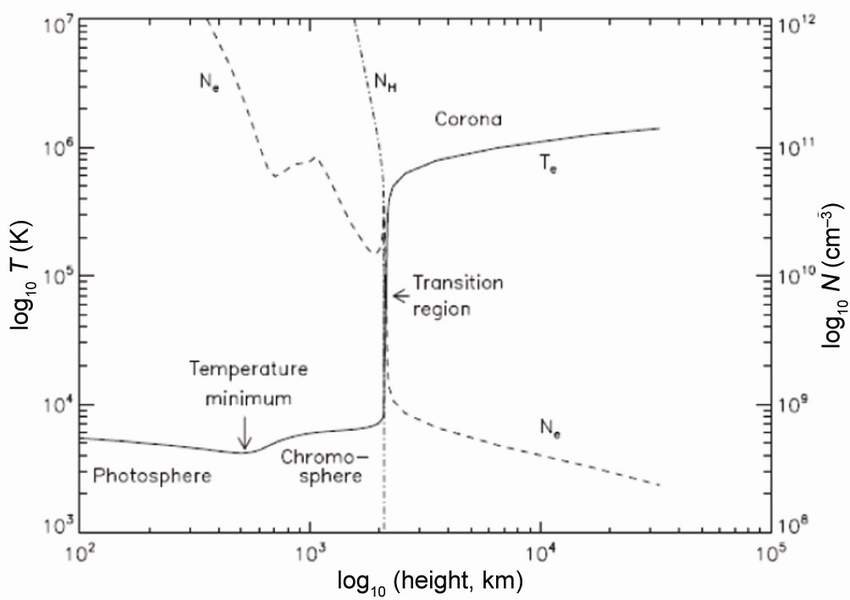
\includegraphics[width=7.5cm]{figures/corona_1d.png}
\caption*{Credits: Aschwanden, 2005}
\end{figure}
\end{minipage}
}
%
%
\frame{
\frametitle{Multi-wavelength view of solar corona}
\begin{figure}
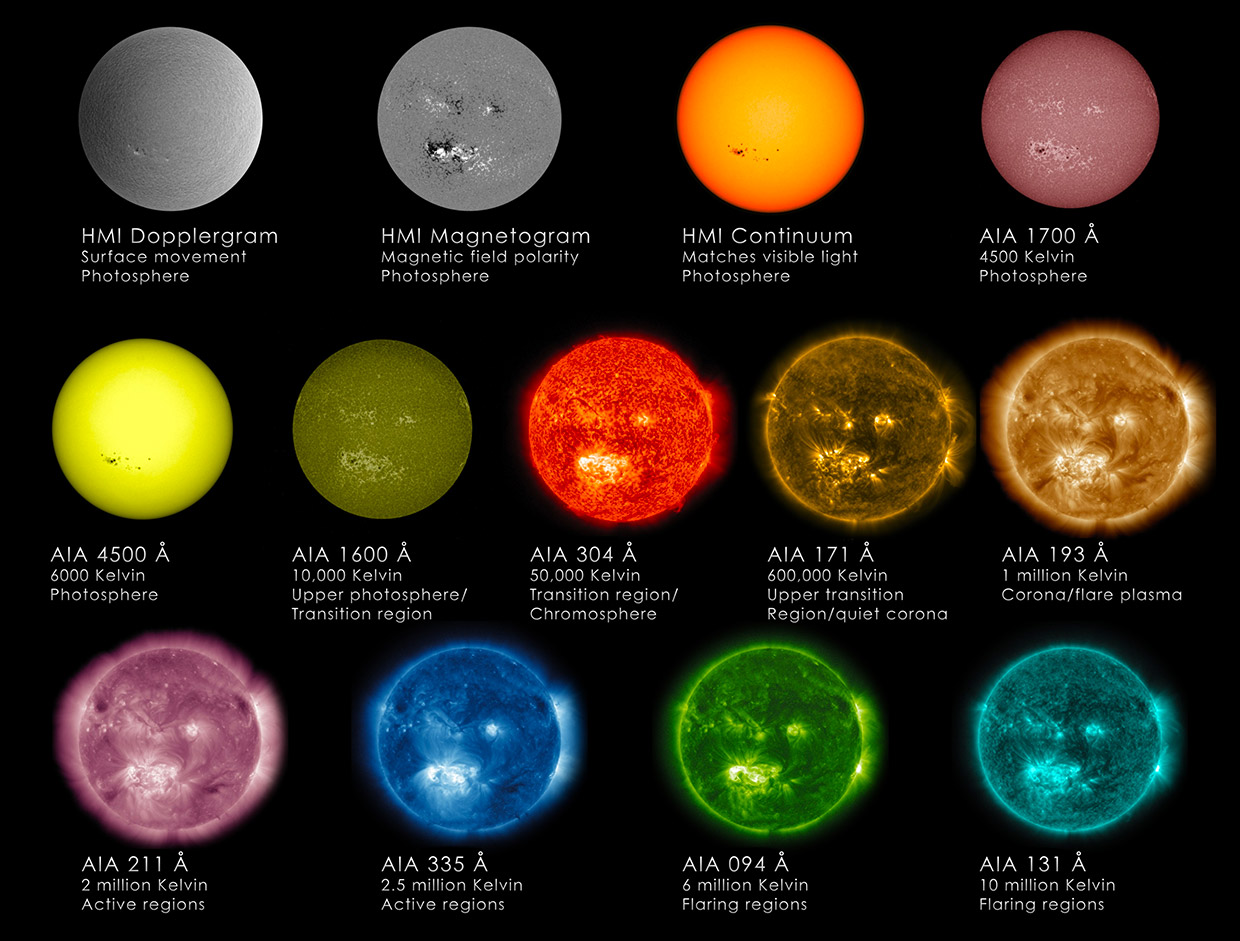
\includegraphics[width=12cm]{figures/sdo-wavelengths-all.jpg}
\caption*{Credits: SDO/NASA}
\end{figure}
}
%
%
\frame{
\frametitle{Coronal structures - prominences}
\begin{minipage}{0.52\linewidth}
\begin{itemize}
\item Right: solar prominences seen ``off-limb''. These are dense plasma structures in the corona that scatter light from the photosphere. 
\item They are much cooler and denser than the corona (approx 10\,000\,kK).
\item How are they supported? Magnetic field of course. 
\item They evolve, become unstable and sometimes explode and give rise to Coronal Mass Ejections (CMEs). \q{Watch the video if there is time}.  
\end{itemize}
\end{minipage}
\begin{minipage}{0.47\linewidth}
\begin{figure}
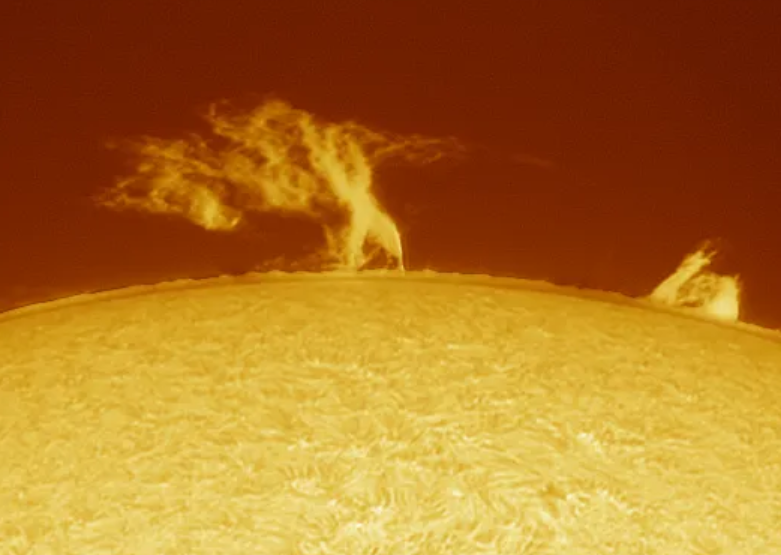
\includegraphics[width=6cm]{figures/prom.png}
\caption*{Credits: André van der Hoeven, HI-Ambacht, The Netherlands. Equipment: Lunt 60/BF1200, NEQ6, DMK21au618}
\end{figure}
\end{minipage}
}
%
%
\frame{
\frametitle{Coronal structures - filaments}
\begin{minipage}{0.52\linewidth}
\begin{itemize}
\item We get another insight into prominences when we see them on limb. 
\item Then they are seen in absorption and are called \textbf{filaments}.
\item \q{Radiative transfer related: why do they look different}?
\item Filaments and prominences are without doubt related to the underlying photospheric magnetic field.
\item Understanding and tracking the structure of filaments and prominences is very important for space weather.
\end{itemize}
\end{minipage}
\begin{minipage}{0.47\linewidth}
\begin{figure}
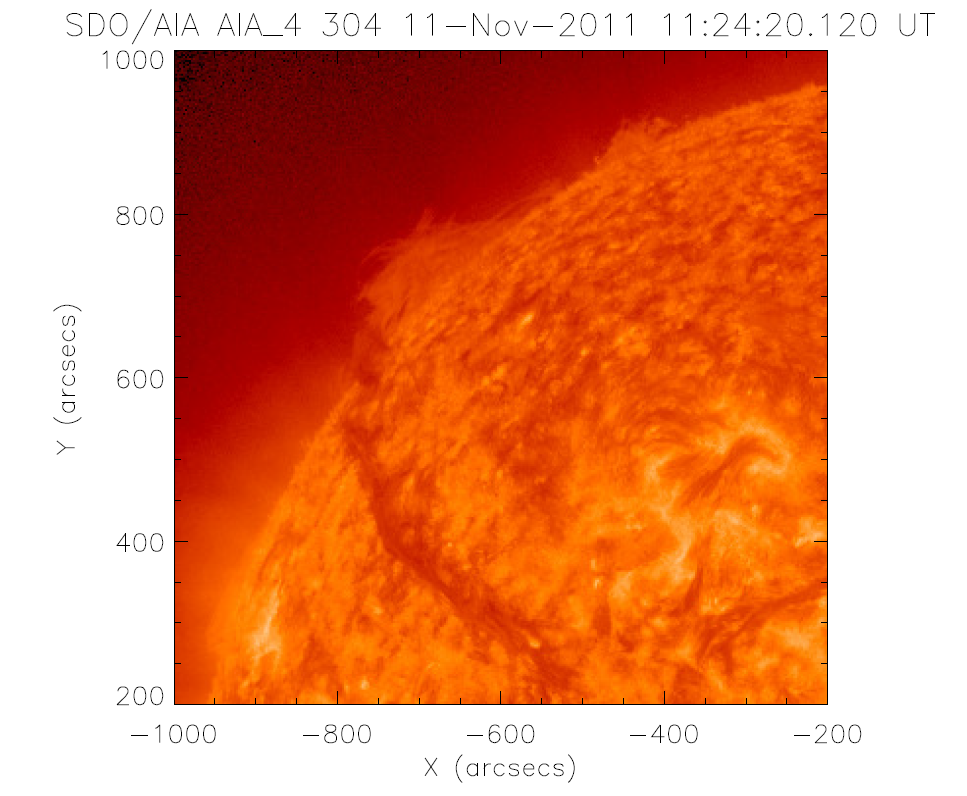
\includegraphics[width=7cm]{figures/promfil.png}
\caption*{Credits: Parenti 2014, SDO/AIA}
\end{figure}
\end{minipage}
}
%
\section{Solar neutrino problem}
\frame{
\frametitle{Solar neutrinos}
\begin{minipage}{0.52\linewidth}
\begin{itemize}
\item There is an ucommon reaction:
\begin{equation}
p^+ + e^{-} + p^+ = D^+ + \nu
\end{equation}
\item Which always produces a neutrino of the same energy equal to 1.442 MeV 
\item These neutrinos are above the treshold of Cl detectors, and can be detected.
\item The solar structure (temperature stratification) determines the flux of these neutrinos. 
\item Predicted capture rate was around 7 snu. 1 snu = 1 capture per second per $10^36$ target atoms. 
\end{itemize}
\end{minipage}
\begin{minipage}{0.47\linewidth}
\begin{figure}
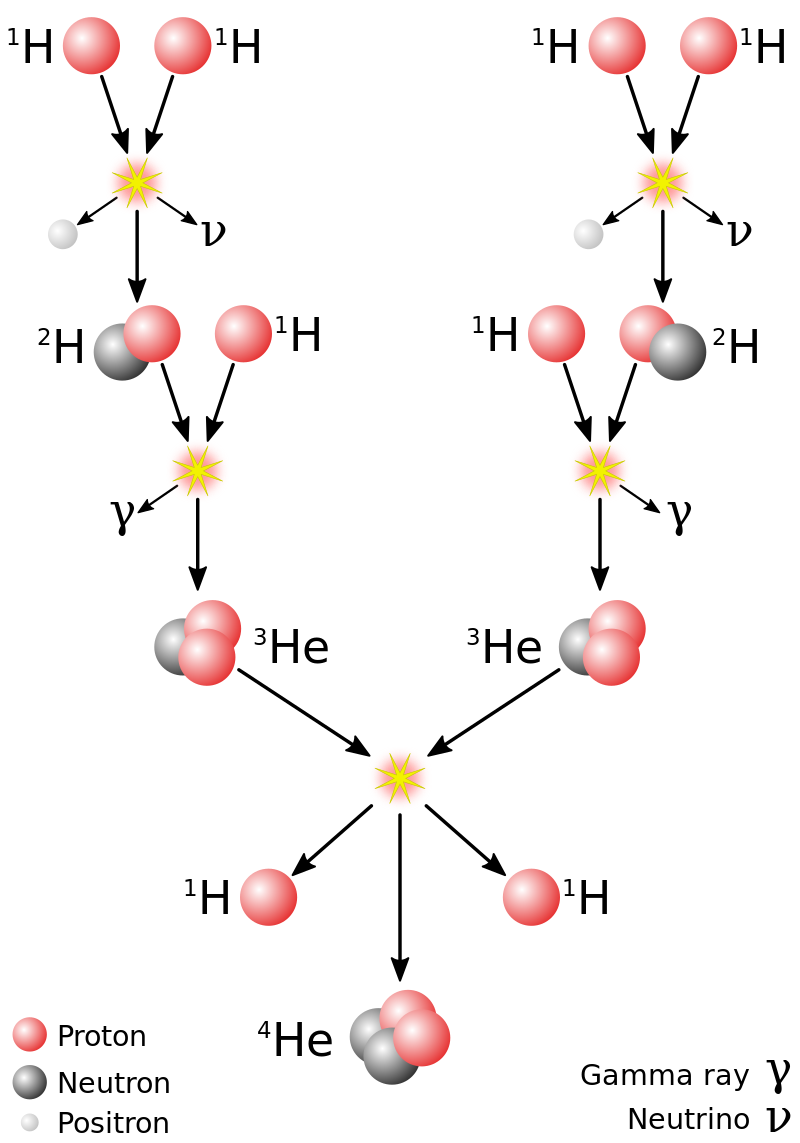
\includegraphics[width=6.5cm]{figures/Fusion_in_the_Sun.png}
\caption*{Credits: Wikipedia}
\end{figure}
\end{minipage}
}
%
\frame{
\frametitle{Solar neutrinos}
\begin{minipage}{0.52\linewidth}
\begin{itemize}
\item Predicted capture rate was around 7 snu. 1 snu = 1 capture per second per $10^36$ target atoms. 
\item Measurement from the experiments at the time (70s) were around \textbf{three times lower}, 2.1 snu.
\item No standard model of the Sun predicted such a low capture rates. 
\item \q{Where can the error be?}
\end{itemize}
\end{minipage}
\begin{minipage}{0.47\linewidth}
\begin{figure}
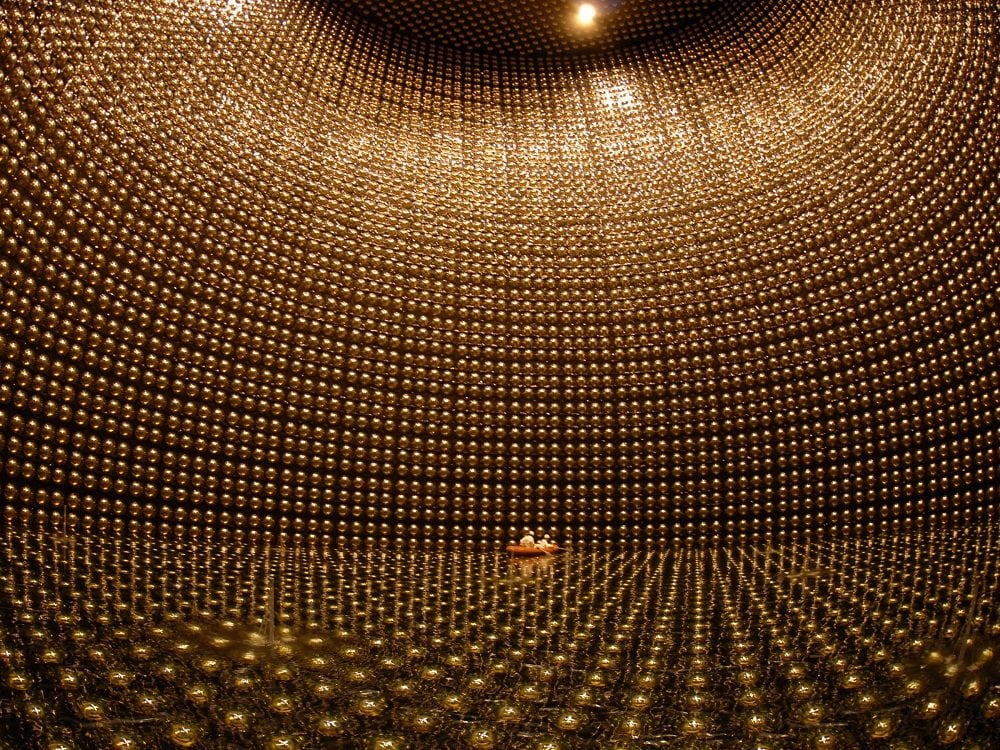
\includegraphics[width=6.5cm]{figures/superk.jpg}
\caption*{Credits: Wikipedia}
\end{figure}
\end{minipage}
}
%
%
\frame{
\frametitle{Solar neutrinos}
\begin{minipage}{0.52\linewidth}
\begin{itemize}
\item Either solar model is wrong. 
\item Or our understanding of neutrino generation is wrong. 
\item Or our instruments are wrong. 
\item Or there is something else that happens with the neutrinos.
\end{itemize}
\end{minipage}
\begin{minipage}{0.47\linewidth}
\begin{figure}
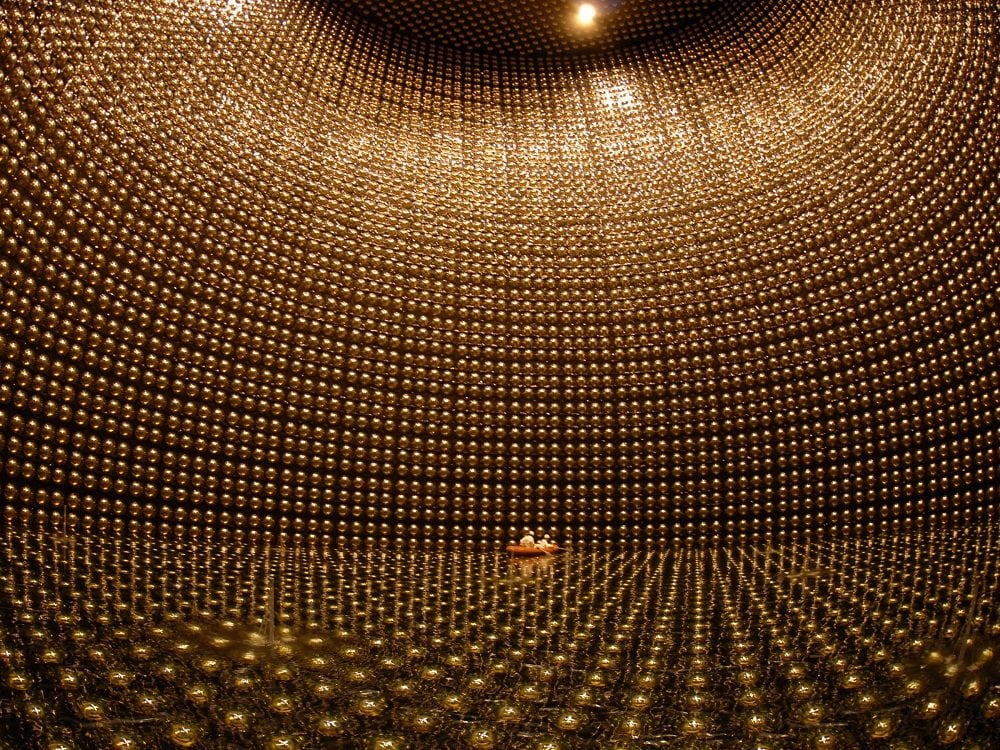
\includegraphics[width=6.5cm]{figures/superk.jpg}
\caption*{Credits: Wikipedia}
\end{figure}
\end{minipage}
}
%
%
\frame{
\frametitle{Solar neutrinos}
\begin{minipage}{0.52\linewidth}
\begin{itemize}
\item Turns out that the neutrinos can undergo oscillations, which was theoretically predicted. 
\item Superkamiokande in 1998 confirmed the existence of neutrino oscillations. 
\item This yielded a Nobel prize for Takaaki Kajita and Arthur McDonald in 2015. 
\item This also meant that the models of solar interior are fine. 
\item It was the \textbf{helioseismology} that allowed us to scrutinize these models and confirm that they are indeed sound and that error lies elsewhere.
\end{itemize}
\end{minipage}
\begin{minipage}{0.47\linewidth}
\begin{figure}
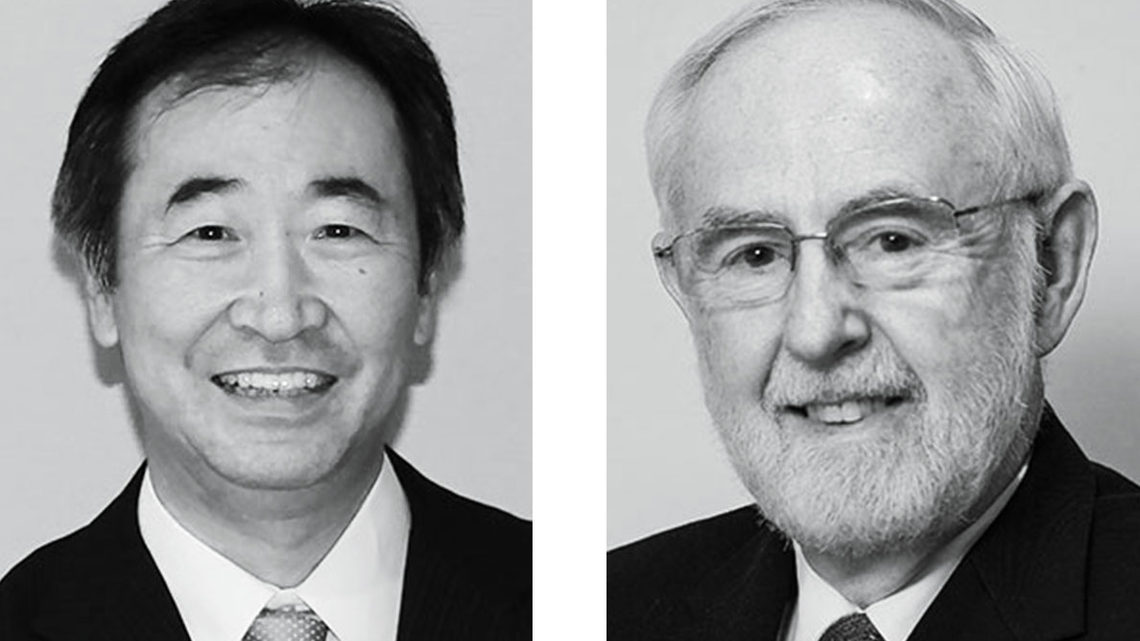
\includegraphics[width=6cm]{figures/award.jpg}\\

\includegraphics[width=6cm]{figures/neutrinoo.png}
\caption*{Credits: NobelPrize.org}
\end{figure}
\end{minipage}
}
%


\section{Conclusions and additional reading}
%
\frame{
\frametitle{Other topics and conclusions}
\begin{itemize}
\item Of course, these are only some topics I have chosen to talk about. Some more interesting solar questions are:
\item What is the nature and origin of sunspots? 
\item Where does the solar magnetic field come from, what is the role of the small-scale dynamo?
\item How do variations in solar irradiance work and how they influence the Earth?
\item What is the mechanism of the solar global dynamo and how does it relate to the flows in the Sun?
\item Can we model and predict the violent solar explosions taking place in the solar atmosphere?
\item Next week, you will hear from Petri about the exicting field or \textbf{helioseismology}, that played a bit role in our studies of the Sun.
\end{itemize}
}

\end{document}
% 

